\documentclass[10pt,a4paper]{article}
\usepackage[margin=25mm,headheight=16pt]{geometry}
\usepackage[T1]{fontenc}
\usepackage[utf8]{inputenc}
\usepackage{helvet}
\renewcommand{\familydefault}{\sfdefault}
\usepackage{amsmath,amssymb,amsthm,booktabs,graphicx,microtype,xcolor,fancyhdr,float}
\usepackage[hidelinks]{hyperref}
\usepackage[numbers]{natbib}
\definecolor{headcolor}{RGB}{0,0,0}
\definecolor{notegray}{RGB}{85,85,85}
\usepackage{titlesec}
\titleformat{\section}{\large\bfseries\color{headcolor}}{\thesection.}{.6em}{}
\titleformat{\subsection}{\normalsize\bfseries\color{headcolor}}{\thesubsection.}{.6em}{}
\titlespacing*{\section}{0pt}{19pt}{8pt}
\titlespacing*{\subsection}{0pt}{13pt}{5pt}
\setlength{\parindent}{0pt}
\setlength{\parskip}{6pt}
\setlength{\emergencystretch}{2em}
\pagestyle{fancy}
\fancyhf{}
\fancyfoot[L]{\scriptsize SENTRY-R: neural proposals and independent privacy-risk audits}
\fancyfoot[R]{\scriptsize\thepage}
\renewcommand{\headrulewidth}{0pt}
\renewcommand{\footrulewidth}{0.2pt}
\theoremstyle{plain}
\newtheorem{proposition}{Proposition}
\newcommand{\E}{\mathbb E}
\newcommand{\Prob}{\mathbb P}
\begin{document}
\vspace*{15mm}
{\color{headcolor}\bfseries\LARGE SENTRY-R: neural proposals and independent audits for privacy-risk release decisions\par}
\vspace{12mm}
{\normalsize Ronald Rethabile Malamule Mahomane\par}
{\small University of Namibia; University of the Witwatersrand; Basis Energy\par}
\vspace{9mm}
{\color{headcolor}\bfseries Abstract\par}
\smallskip
A release committee needs an explicit rule for deciding when the estimated
success probability of a declared privacy attack is acceptable. A neural score
alone cannot provide that rule. We propose SENTRY-R (scenario-enriched neural
triage for release review), a workflow in which language models suggest attack
scenarios, measured
development attacks train a multi-output deep network, and an independent
simultaneous audit decides release eligibility. For each candidate, risk is a
vector indexed by adversary, harm, target group and release vintage, with a
separate pooled-release attack. We derive the counted-outcome learning objective
and backpropagation, then show that exact binomial upper bounds control the
chance of any false certification across a finite shortlist even after
adaptive development and utility-based final choice. On a synthetic toy law,
over ten seeded replicates, a logistic model trained to convergence has
slightly lower held-out log loss than a three-layer network in every
replicate. The comparison shows that the software runs; it shows no gain from
depth and no performance on real release programmes. The workflow exposes what a language
model may change, what requires observed attack data, and which assumptions a
release decision must record.

{\small\textbf{Keywords:} statistical disclosure control; release governance;
record linkage; neural risk model; language model; simultaneous inference.\par}
\vspace{5mm}
{\scriptsize\color{notegray}Author manuscript; not a BIS or IFC publication.
The views are the author's own.\par}

\section{The release problem}

Statistical agencies and central banks publish data because they have public
value, but overlapping releases and auxiliary information may make records
linkable. A reciprocal key frequency can quantify identification under a
specific matching model \citep{fellegi1969}; it cannot silently stand in for
every adversary, target group, time period or harm. Repeated access gives an
attacker a different experiment from the one-release analysis. The underlying
privacy-risk study examines this difference with a 200,000-record synthetic
register, a granular credit-register simulation, two public microdata files and
pooled-vintage attacks. Those empirical results precede the neural extension;
none is a held-out evaluation of its deep model. The underlying derivations,
experimental detail and caveats are provided in the accompanying full
manuscript, \emph{Governing privacy risk across repeated statistical releases:
probability models, programme tolerances and accountable decisions}.

The added problem is methodological: how can an institution search a large
family of release settings and adversaries while preserving a decision rule
whose error rate survives that search? We specify a trainable proposal model
and an independent audit. Utility remains an institutional value, whereas a
policy tolerance is declared and signed by its owner. The price of harm and
the value of the release can inform that tolerance \citep{abowd2019}; a
network cannot choose its legitimacy.

\section{A risk vector with a declared sampling law}

Let $\theta$ be a candidate release mechanism and
$j=(a,h,g,v)\in\mathcal J$ encode an adversary, harm, target group and
vintage. A pooled-vintage attack gets its own coordinate. The scenario
specifies a binary success function $s_{\theta j}$ and a full law
$P_{\theta j}$ for a fresh target, auxiliary information and attack
randomness. Its risk and policy tolerance are
\begin{equation}
 r_j(\theta)=\E_{P_{\theta j}}s_{\theta j}(Z),\qquad
 \tau_j\in(0,1),\qquad |\mathcal J|=n.
 \label{eq:ifc-risk}
\end{equation}
A target-level probability and a group average are different estimands;
both need their own scenario. After independent final audits yield simultaneous
upper bounds $\overline r_{\theta j}$, define the audited margin vector and
its minimum
\begin{equation}
 z_j(\theta)=1-\frac{\overline r_{\theta j}}{\tau_j},\quad
 \boldsymbol z(\theta)\in\mathbb R^n,\quad
 T(\theta)=\min_j z_j(\theta).
 \label{eq:ifc-position}
\end{equation}
Release eligibility requires $T(\theta)\geq0$ and the full vector must be
reported. An unaudited declared coordinate receives upper bound one and fails
when $\tau_j<1$. The rule starts with no inherited claim of safety.

\section{Scenario expansion and the deep proposal model}

An LLM can suggest a new pooled attack or auxiliary information pattern.
SENTRY-R treats its text and numeric features as \emph{untrusted proposals}:
a fixed schema checks names and ranges. The calling code records the model
name and a hash of the exact prompt; the model's output cannot set these
fields.
A separate experiment observes successes $K_{ij}$ in $B_{ij}$ development
attack trials. No generated success label can enter the training set.
The validator and measured outcome are joined by a proposal digest. Human
review remains responsible for the scenario's plausibility, lawful data access
and sampling unit.

In a repeatable round, the analyst (i) freezes a feature and coordinate schema;
(ii) accepts or rejects an LLM-suggested scenario with a recorded reason;
(iii) runs the declared attack and writes independent development counts;
(iv) appends measured rows to a new training version; and (v) evaluates on
whole programmes omitted from training. Before any final audit, the software
writes one hashed record that fixes the shortlist, $\alpha$, the planned
sample size of every audited coordinate, the tolerance owner, an expiry date
and the identifiers of all development evidence. The audit reads $\alpha$
from that record and refuses a changed record, a lapsed expiry date, a trial
count that departs from the plan, and evidence already used in development.
An optional append-only ledger refuses a second audit of the same record.
These checks bind an audit to its record. They do not prove what happened
first: the hash has no key or trusted time stamp, and nothing stops an
analyst from writing a new record or a new ledger. These steps permit many rounds of
model improvement without making the subsequent confidence statement depend
on a generated answer.

For $x_i\in\mathbb R^d$ and $L$ ReLU hidden layers, the multi-output predictor is
\begin{equation}
 h_i^0=x_i,\quad h_i^{\ell+1}=\max\{0,h_i^\ell W_\ell+b_\ell\},\quad
 \widehat{\boldsymbol r}_\phi(x_i)=
 \sigma(h_i^L W_{\rm o}+b_{\rm o})\in(0,1)^n.
 \label{eq:ifc-net}
\end{equation}
Depth zero is logistic regression. Training minimises counted binomial negative
log likelihood plus a declared ridge penalty:
\begin{equation}
 \mathcal L(\phi)=
 -\frac{1}{\sum_{ij}B_{ij}}\sum_{ij}
 \left[K_{ij}\log p_{ij}+(B_{ij}-K_{ij})\log(1-p_{ij})\right]
 +\frac\lambda2\sum_\ell\|W_\ell\|_F^2.
 \label{eq:ifc-loss}
\end{equation}
If $K_{ij}\mid x_i,B_{ij}\sim\mathrm{Binom}(B_{ij},\pi_j(x_i))$ and the
trial count was chosen before observing successes, the conditional expected
unregularised loss is minimised at $p_{ij}=\pi_j(x_i)$: its excess is a
positive multiple of
$D_{\rm KL}(\mathrm{Bern}(\pi_j)\|\mathrm{Bern}(p_{ij}))$.
With $P=(p_{ij})$, the logit derivative is
$(B\odot P-K)/\sum_{ij}B_{ij}$; multiplying backward through $W_\ell^\top$
and the ReLU indicator gives every hidden-layer gradient. This derivation
states precisely what the software trains. Calibration on a held-out
\emph{programme} diagnoses prediction; it does not certify a new target
\citep{guo2017}.

\begin{figure}[H]
\centering
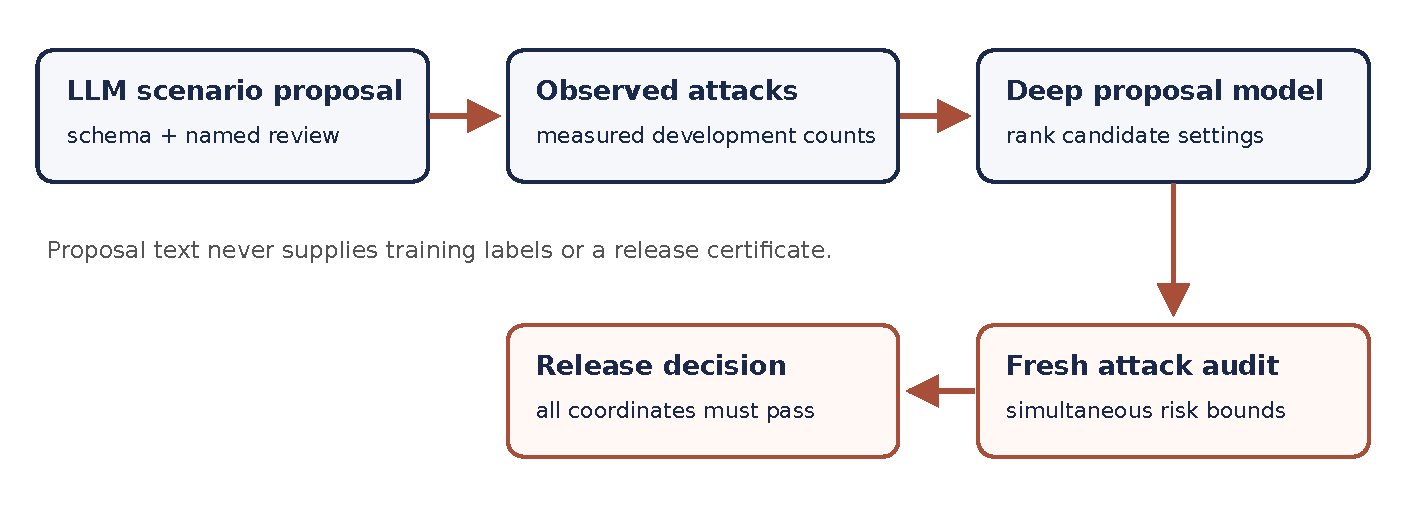
\includegraphics[width=.95\linewidth]{diagrams/sentry_r_loop.pdf}
\caption{The scenario proposal changes development work. A separate final attack audit decides release eligibility.}
\label{fig:ifc-workflow}
\end{figure}

\section{Independent audit and finite-family guarantee}

The network ranks a fixed shortlist $\Theta_0$ of $C$ candidates using the
largest predicted risk-to-tolerance ratio. For every $(\theta,j)$, freeze
$B_{\theta j}$ and draw fresh, conditionally independent attacks; let
$K_{\theta j}$ succeed. With $M=Cn$ and $\gamma=\alpha/M$, define the exact
one-sided binomial upper bound \citep{clopper1934}
\begin{equation}
 \overline r_{\theta j}=
 \begin{cases}
 1,&K_{\theta j}=B_{\theta j},\\
 F^{-1}_{\mathrm{Beta}(K_{\theta j}+1,B_{\theta j}-K_{\theta j})}
 (1-\gamma),&K_{\theta j}<B_{\theta j}.
 \end{cases}
 \label{eq:ifc-bound}
\end{equation}
The bound includes, rather than estimates away, final attack-draw uncertainty.

\begin{proposition}[Selection after adaptive development]
Let $\mathcal D$ contain all development information, including repeated
LLM proposals, observed development attacks, fitted models and the shortlist.
Conditional on $\mathcal D$, fix the release, scenarios, $C$, $n$ and each
sample size. If each final count has law
$K_{\theta j}\mid\mathcal D\sim\mathrm{Binom}(B_{\theta j},r_j(\theta))$,
then selecting any candidate with $T(\theta)\geq0$, including the most useful
eligible candidate, has probability at most $\alpha$ of accepting any candidate
whose actual declared risk exceeds a tolerance.
\end{proposition}
\begin{proof}
For a fixed risk $p$ and count $k<b$, the binomial lower tail
$F_p(k)=\sum_{t=0}^k\binom bt p^t(1-p)^{b-t}$ decreases with $p$.
Its inversion yields \eqref{eq:ifc-bound} and satisfies
$\Prob_p\{p>\overline r(K)\}\leq\gamma$. Conditional on $\mathcal D$,
a union bound across the $Cn$ pairs gives simultaneous coverage at least
$1-\alpha$, without requiring independence across pairs. On that event every
eligible candidate meets every tolerance, however the final eligible one is
chosen. Averaging over $\mathcal D$ gives the unconditional statement.
\end{proof}

At zero observed successes,
$\overline r=1-\gamma^{1/B}$. A coordinate can pass tolerance $\tau$
with zero successes exactly when
\begin{equation}
 B\geq\left\lceil\frac{\log(\alpha/(Cn))}{\log(1-\tau)}\right\rceil.
 \label{eq:ifc-budget}
\end{equation}
For $C=4$, $n=2$, $\alpha=.05$ and $\tau=.12$, this is 40 independent
trials per coordinate, or 320 if all eight coordinates receive the same
budget. A positive success count can require more. Reusing one auxiliary
file across nominal trials, sampling finite targets without replacement, or
learning from final audit outcomes requires another valid design.

\clearpage
\section{Scale, demonstration and evidence limits}

A width-$q$, depth-$L$ dense model uses
$O(dq+(L-1)q^2+qn)$ parameters and forward operations for $L\geq1$.
At $N$ rows and $E$ epochs training is
$O(EN[dq+(L-1)q^2+qn])$. This does not reduce the $Cn$ simultaneous
confidence limits or the attack trials behind them. Even if a true risk
function is Lipschitz in $d$ features, a direct accuracy-$\epsilon$ grid
can require order $(L_0/\epsilon)^d$ cells for Lipschitz constant $L_0$.
Network capacity alone does not remove this dimensional cost.

The package includes a \emph{synthetic} comparison with six input features
and two risk coordinates (Table \ref{tab:sentry-synthetic}). For each of ten
seeds it draws three disjoint toy programmes: 320 counted training rows, 100
rows used only for early stopping and 2,000 rows used only to report the
loss. A logistic model and a three-hidden-layer ReLU model train on identical
trials until 150 epochs pass without improvement; no best epoch reaches the
cap. The logistic model has slightly lower test log loss in all ten
replicates, and the mean gap is smaller than the spread across replicates.
The table shows that the pipeline runs, not that depth helps.
\begin{table}[H]
\centering
\small
\caption{Synthetic SENTRY-R comparison over 10 seeded replicates of the toy law. Each replicate draws 320 training rows, 100 rows used only for early stopping (patience 150 epochs, cap 6000) and 2000 test rows used only for the reported losses. Entries are mean (standard deviation) across replicates; smaller is better. The last row is the paired deep-minus-logistic test log loss (range 0.0004 to 0.0050; deep lower in 0 of 10). These are not results on real release programmes.}
\label{tab:sentry-synthetic}
\begin{tabular}{lrrr}
\toprule
Proposal model & Test log loss & Test Brier score & Best epoch (range) \\
\midrule
Logistic & 0.2556 (0.0043) & 0.0727 (0.0017) & 404--898 \\
Three-layer ReLU & 0.2576 (0.0047) & 0.0735 (0.0018) & 79--402 \\
\midrule
Deep minus logistic & 0.0020 (0.0014) & & \\
\bottomrule
\end{tabular}
\end{table}

These are properties of a designed toy law, whose test programmes share the
training law and feature range, and say nothing about accuracy on
confidential or public microdata. A valid assessment must hold out
whole real release programmes, compare worst-group calibration and utility at
fixed audit budgets, and repeat pooled-vintage attacks. The existing
credit-register and public-file results cannot be re-labelled as evidence for
the new model.

A shift in the full attack-draw law from $P_{\theta j}$ to $Q_{\theta j}$
with justified total-variation bound $\delta_{\theta j}$ permits
$r_{Q_{\theta j}}(\theta)\leq\overline r_{\theta j}+\delta_{\theta j}$
(up to one) on the same simultaneous coverage event. A change in an embedding
is not itself such a bound. Missing attacks, future auxiliary files and
out-of-scope input values must be recorded as gaps, not assigned a reassuring
predicted probability.

\section{Implications for a release committee}

The model is a search instrument. Its model file records the feature schema,
training-only scaling, weights, training and validation hashes and held-out
loss. A frozen shortlist records its own digest, $\alpha$, the planned trials,
the tolerance owner and the expiry date. The decision record then contains
every observed audit count, upper bound, risk coordinate, tolerance, utility,
owner and expiry. Only measured development attacks can update the
network; only fresh final audits can pass the release gate. This division makes
an LLM useful for widening scrutiny without granting its generated answer
authority over confidential-data release. Source, tests, sample commands and
an editable workflow diagram accompany the longer mathematical manuscript.

\begin{thebibliography}{9}\small
\bibitem{abowd2019} Abowd, J. M. and Schmutte, I. M. (2019), ``An economic analysis of privacy protection and statistical accuracy as social choices'', \emph{American Economic Review} 109(1), 171--202.
\bibitem{clopper1934} Clopper, C. J. and Pearson, E. S. (1934), ``The use of confidence or fiducial limits illustrated in the case of the binomial'', \emph{Biometrika} 26(4), 404--413.
\bibitem{fellegi1969} Fellegi, I. P. and Sunter, A. B. (1969), ``A theory for record linkage'', \emph{Journal of the American Statistical Association} 64(328), 1183--1210.
\bibitem{guo2017} Guo, C., Pleiss, G., Sun, Y. and Weinberger, K. Q. (2017), ``On calibration of modern neural networks'', \emph{Proceedings of Machine Learning Research} 70, 1321--1330.
\end{thebibliography}
\end{document}
